\section{Results}
% \begin{table}[htbp]
% \centering
% \begin{tabular}{llll}
%  & & \multicolumn{2}{c}{\textbf{All CKD stage 3-5 (n=10179)}}\\
% \hline
% \textbf{Characteristics} & \textbf{All CKD (n=22336)} & \textbf{Non-ESRD (n=2790)}& \textbf{ESRD (n=7389)}\\
% \hline
% \multicolumn{4}{l}{\textbf{Demographics}} \\
% Age (years) & 71.1 $\pm$ 14.3 & 74.795 $\pm$ 12.470& 71.774 $\pm$ 13.668\\
% Gender & M: 13223, F: 9113 & M: 1555, F:1235& M: 4247, F: 3142\\
% \hline
% \multicolumn{4}{l}{\textbf{Clinical Characteristics}} \\
% CKD Stage 3-5, n (\%) & 10179 (45.6) & -& -\\
% Hypertension, n (\%) & 10531 (47.1) & 1418  (50.824)& 4317 (58.425)\\
% Diabetes Mellitus, n (\%) & 4954 (22.2) & 565 (20.251)& 2288 (30.965)\\
% \hline
% \multicolumn{4}{l}{\textbf{Laboratory Parameters}} \\
% Serum Creatinine (mg/dL) & 2.256 $\pm$ 1.756 & 2.126 $\pm$ 2.026& 2.27 $\pm$ 1.723\\
% eGFR (mL/min/1.73m²) & 41.502 $\pm$ 23.532 & 46.4 $\pm$ 24.35& 40.968 $\pm$ 23.379\\
% Proteinuria (g/24 hours) & 0.836 (2.474)* & 0.837 (2.294)*& 0.458 (4.319)*\\
% \hline
% \multicolumn{4}{l}{\textbf{Medication Use}} \\
% ACE Inhibitors or ARBs, n (\%) & 8633 (38.7) & 954 (34.194)& 3221 (43.592)\\
% \hline
% \multicolumn{4}{l}{\small *Values presented as median (IQR)} \\
% \end{tabular}
% \caption{Baseline Characteristics by ESRD Status. Patients are stratified by whether they developed ESRD during follow-up. We investigate a wide variety of useful features defined by \citep{zhong2017perspective_CKD_biomarkers} and more recently \citep{dana2024integratedmachinelearningsurvival_feature_analysis}. We investigate these features across time. We also investigate features that may not necessarily be omnipresent across all time points.}
% \label{tab:baseline_characteristics}
% \end{table}

\begin{table}[h]
\centering
\resizebox{0.5\textwidth}{!}{%
\begin{tabular}{lcc}
\hline
\textbf{} & \textbf{Non-ESRD} & \textbf{ESRD} \\
\hline
\multicolumn{3}{l}{\textbf{Patient Demographics}} \\
\quad \# of Patients & 2,790 & 7,389 \\
\quad Age (years) & 74.8 ± 12.5 & 71.8 ± 13.7 \\
\quad Male & 55.7\% & 57.5\% \\
\quad Hypertension & 50.8\% & 58.4\% \\
\quad Diabetes mellitus & 20.3\% & 31.0\% \\
\quad ACE inhibitor/ARB use & 34.2\% & 43.6\% \\
\quad \# of admissions & 6,773& 47,441\\
\hline
\multicolumn{3}{l}{\textbf{Laboratory Values}} \\
\quad Serum creatinine (mg/dL) & 2.1 ± 2.0 & 2.3 ± 1.7 \\
\quad eGFR (mL/min/1.73m²) & 46.4 ± 24.4 & 41.0 ± 23.4 \\
\quad Proteinuria (g/24h)* & 0.8 [2.3] & 0.5 [4.3] \\
\hline
\end{tabular}%
}
\caption{Baseline Characteristics of CKD Stage 3-5 Patients by ESRD Status. This analysis focuses exclusively on patients with chronic kidney disease stages 3-5 (n=10,179), stratified by whether they developed end-stage renal disease (ESRD) during follow-up. Continuous variables are presented as mean ± standard deviation, except for proteinuria which is presented as median with interquartile range due to its skewed distribution. We investigate a wide variety of useful features defined by \citep{zhong2017perspective_CKD_biomarkers} and more recently \citep{dana2024integratedmachinelearningsurvival_feature_analysis}. We investigate these features across time. We also investigate features that may not necessarily be omnipresent across all time points.}
\label{tab:baseline_characteristics}
\end{table}

\subsection{Dataset Statistics}
Given that ESRD risks are substantially higher in later CKD stages \citep{sud2014ckd_esrd_at_stage3_5}, we identified 10,179 patients with stage 3--5 CKD, of whom 7,389 progressed to ESRD. As shown in Table~\ref{tab:baseline_characteristics}, ESRD patients were younger, had higher rates of diabetes and hypertension, more severe renal dysfunction, and increased use of renin--angiotensin inhibitors compared to non-progressors, establishing clinically meaningful baseline differences for model comparison.

\textbf{Evaluation metrics.} We benchmark our survival analysis models using three conventional metrics: concordance index (C-index) \citep{longato2020practical_c_index}, Brier score \citep{assel2017brier}, and area under the ROC curve (AUC) \citep{huang2005using_AUC}.

\subsection{Time Invariant}
We benchmark several traditional time-invariant models for CKD survival analysis as discussed in Section \ref{sec:models}. Specifically, we evaluate traditional models (Cox proportional hazards, Weibull), ensemble methods (gradient boosted survival analysis or GBSA, survival random forests or SRF), and the neural network-based DeepSurv model.

% Time-Invariant Models Table
% \begin{table}[h!]
%     \centering
%     \begin{tabular}{lccc}
%         \toprule
%         \textbf{Model} & \textbf{C-Index} & \textbf{Brier score} & \textbf{AUC} \\
%         \midrule
%         Cox & 0.517±0.008  &   0.443±0.001   &  0.527±0.012 \\
%         DeepSurv & \textbf{0.523±0.002}   &  0.475±0.012  &   0.464±0.002 \\
%         GBSA & 0.523±0.011  &   0.329±0.043   &  0.534±0.016 \\
%         SRF & 0.517±0.006  &   0.502±0.004  &   0.527±0.009 \\
%         Weibull & 0.521±0.001   &  0.485±0.007   &  \textbf{0.535±0.001} \\
%         LogisticHazard & 0.514±0.010  &   \textbf{0.566±0.008}  &   0.496±0.023 \\
%         Fast Survival SVM & 0.510±0.007  &   0.252±0.004  &   0.485±0.010 \\
%         \bottomrule
%     \end{tabular}
%     \caption{Performance of Time-Invariant Models. Models use static patient snapshots without longitudinal information. Bold values indicate best performance for each metric.}
%     \label{tab:time_invariant_performance}
% \end{table}
\begin{table}[h!]
    \centering
    \footnotesize % Smaller font size
    \resizebox{0.5\textwidth}{!}{% Resize to fit textwidth
    \begin{tabular}{@{}lccc@{}}
        \toprule
        \textbf{Model} & \textbf{C-Index} $\uparrow$ & \textbf{Brier score} $\downarrow$ & \textbf{AUC} $\uparrow$ \\
        \midrule
        Cox & 0.517±0.008 & 0.443±0.001 & 0.527±0.012 \\
        DeepSurv & \textbf{0.523±0.002} & 0.475±0.012 & 0.464±0.002 \\
        GBSA & 0.523±0.011 & 0.329±0.043 & 0.534±0.016 \\
        SRF & 0.517±0.006 & 0.502±0.004 & 0.527±0.009 \\
        Weibull & 0.521±0.001 & 0.485±0.007 & \textbf{0.535±0.001} \\
        LogisticHazard & 0.514±0.010 & 0.566±0.008 & 0.496±0.023 \\
        Fast Survival SVM & 0.510±0.007 & \textbf{0.252±0.004} & 0.485±0.010 \\
        \bottomrule
    \end{tabular}
    } % End resizebox
    \caption{Performance of Time-Invariant Models. Models use static patient snapshots without longitudinal information. Bold values indicate best performance for each metric.}
    \label{tab:time_invariant_performance}
\end{table}

\textbf{More complex and less interpretable models do not provide any significant benefits in time invariant settings.} At the cost of explainability, we see a small improvement in DeepSurv over the Cox model in C-index. However, the interpretable Weibull model is comparable and better depending on the metric. Nonetheless, traditional models like the Cox or Weibull model seem comparable in performance to the less interpretable SRF, GBSA, and DeepSurv models when considering both metrics.


\subsection{Time Variant and Heterogeneous Scenarios}
To understand the predictive capababilites of survival analysis models under different time variant settings, we benchmarked 4 models. Namely, we benchmark the Cox model, and a variety of deep architectures such as Dynamic-DeepHit \citep{lee2019dynamic_deephit}, Hazard Transformer \citep{hazard_transformer}, and RNN-Surv \citep{martinez2020rnnsurv}. 

\begin{table}[h!]
    \centering
    \footnotesize
    \resizebox{0.5\textwidth}{!}{%
    \begin{tabular}{@{}l*{3}{c}@{}}
        \toprule
        \multicolumn{4}{c}{\textbf{Time-Variant (Baseline)}} \\
        \midrule
        \textbf{Model} & \textbf{C-Index} $\uparrow$ & \textbf{Brier} $\downarrow$ & \textbf{AUC} $\uparrow$ \\
        \midrule
        Cox & 0.545±0.001 & 0.215±0.002 & 0.539±0.002 \\
        Dynamic-DeepHit & \textbf{0.735±0.069} & \textbf{0.036±0.003} & \textbf{0.798±0.197} \\
        Hazard Transformer & 0.500±0.000 & 0.566±0.007 & 0.500±0.000 \\
        RNNSurv & 0.640±0.076 & 0.082±0.088 & 0.648±0.080 \\
        Logistic Hazard & 0.514±0.010 & 0.566±0.008 & 0.496±0.023 \\
        \midrule
        \multicolumn{4}{c}{\textbf{Time-Variant Raw}} \\
        \midrule
        \textbf{Model} & \textbf{C-Index} $\uparrow$ & \textbf{Brier} $\downarrow$ & \textbf{AUC} $\uparrow$ \\
        \midrule
        Cox & \textcolor{red}{0.374±0.004} $\downarrow$ & \textcolor{red}{0.926±0.029} $\uparrow$ & \textcolor{red}{0.352±0.004} $\downarrow$ \\
        Dynamic-DeepHit & \textcolor{green}{0.780±0.065} $\uparrow$ & \textcolor{gray}{0.037±0.002} $=$ & \textcolor{green}{0.830±0.187} $\uparrow$ \\
        Hazard Transformer & \textcolor{gray}{0.500±0.000} $=$ & \textcolor{gray}{0.566±0.007} $=$ & \textcolor{gray}{0.500±0.000} $=$ \\
        RNNSurv & \textcolor{green}{0.668±0.042} $\uparrow$ & \textcolor{gray}{0.096±0.057} $=$ & \textcolor{green}{0.681±0.040} $\uparrow$ \\
        Logistic Hazard & \textcolor{gray}{0.507±0.016} $=$ & \textcolor{gray}{0.566±0.007} $=$ & \textcolor{gray}{0.513±0.021} $=$ \\
        \midrule
        \multicolumn{4}{c}{\textbf{Heterogeneous Features}} \\
        \midrule
        \textbf{Model} & \textbf{C-Index} $\uparrow$ & \textbf{Brier} $\downarrow$ & \textbf{AUC} $\uparrow$ \\
        \midrule
        Cox & \textcolor{red}{0.406±0.003} $\downarrow$ & \textcolor{red}{0.294±0.007} $\uparrow$ & \textcolor{red}{0.389±0.003} $\downarrow$ \\
        Dynamic-DeepHit & \textcolor{green}{0.761±0.014} $\uparrow$ & \textcolor{red}{0.056±0.000} $\uparrow$ & \textcolor{red}{0.492±0.047} $\downarrow$ \\
        Hazard Transformer & \textcolor{gray}{0.500±0.000} $=$ & \textcolor{red}{0.546±0.000} $\downarrow$ & \textcolor{gray}{0.500±0.000} $=$ \\
        RNNSurv & \textcolor{green}{0.647±0.002} $\uparrow$ & \textcolor{red}{0.127±0.043} $\uparrow$ & \textcolor{green}{0.651±0.003} $\uparrow$ \\
        Logistic Hazard & \textcolor{gray}{0.518±0.008} $=$ & \textcolor{red}{0.529±0.027} $\uparrow$ & \textcolor{gray}{0.526±0.015} $=$ \\
        \bottomrule
    \end{tabular}
    }
    \caption{Stacked Performance Comparison Across Settings. Time-Variant serves as baseline. Green indicates improvement ($>0.02$ difference), red indicates degradation ($>0.02$ difference), gray indicates no significant change ($\leq 0.02$ difference). For C-Index and AUC, higher is better ($\uparrow$); for Brier score, lower is better ($\downarrow$). Dynamic-DeepHit shows consistent strong performance across all settings and sees upwards of a 4\% performance improvement in the raw setting.}
    \label{tab:stacked_performance_comparison}
\end{table}

% \begin{table*}[h!]
%     \centering
%     \footnotesize
%     \resizebox{\textwidth}{!}{%
%     \begin{tabular}{@{}l*{6}{c}@{}}
%         \toprule
%         & \multicolumn{3}{c}{\textbf{Time-Variant}} & \multicolumn{3}{c}{\textbf{Time-Variant Raw}} \\
%         \cmidrule(lr){2-4} \cmidrule(lr){5-7}
%         \textbf{Model} & \textbf{C-Index} $\uparrow$ & \textbf{Brier} $\downarrow$ & \textbf{AUC} $\uparrow$ & \textbf{C-Index} $\uparrow$ & \textbf{Brier} $\downarrow$ & \textbf{AUC} $\uparrow$ \\
%         \midrule
%         Cox & 0.545±0.001 & 0.215±0.002 & 0.539±0.002 & 0.374±0.004 & 0.926±0.029 & 0.352±0.004 \\
%         Dynamic-DeepHit & \textbf{0.735±0.069} & \textbf{0.036±0.003} & \textbf{0.798±0.197} & \textbf{0.780±0.065} & \textbf{0.037±0.002} & \textbf{0.830±0.187} \\
%         Hazard Transformer & 0.500±0.000 & 0.566±0.007 & 0.500±0.000 & 0.500±0.000 & 0.566±0.007 & 0.500±0.000 \\
%         RNNSurv & 0.640±0.076 & 0.082±0.088 & 0.648±0.080 & 0.668±0.042 & 0.096±0.057 & 0.681±0.040 \\
%         Logistic Hazard & 0.514±0.010 & 0.566±0.008 & 0.496±0.023 & 0.507±0.016 & 0.566±0.007 & 0.513±0.021 \\
%         \bottomrule
%     \end{tabular}
%     }
%     \caption{Performance of Longitudinal Models: Time-Variant vs Time-Variant Raw. Time-variant include eGFR across multiple time points. Time-variant raw decomposes eGFR into its input components and feeds those into the models. Dynamic-DeepHit performs best across both settings.}
%     \label{tab:time_variant_performance}
% \end{table*}
% \begin{table}[h!]
%     \centering
%     \footnotesize
%     \resizebox{0.5\textwidth}{!}{%
%     \begin{tabular}{@{}l*{3}{c}@{}}
%         \toprule
%         \textbf{Model} & \textbf{C-Index} $\uparrow$ & \textbf{Brier} $\downarrow$ & \textbf{AUC} $\uparrow$ \\
%         \midrule
%         Cox & 0.406±0.003  &   0.294±0.007   &  0.389±0.003 \\
%         Dynamic-DeepHit & \textbf{0.761±0.014}  &   \textbf{0.056±0.000}  &   0.492±0.047 \\
%         Hazard Transformer & 0.500±0.000 & 0.546±0.000 & 0.500±0.000 \\
%         RNNSurv & 0.647±0.002  &   0.127±0.043  &   \textbf{0.651±0.003} \\
%         Logistic Hazard & 0.518±0.008  &   0.529±0.027  &   0.526±0.015 \\
%         \bottomrule
%     \end{tabular}
%     }
%     \caption{Performance of Longitudinal Models: Heterogeneous Setting. This setting incorporates heterogeneous features like Albumin and protein measurements alongside eGFR. RNNSurv performs best for C-Index and AUC, while Cox regression achieves the best Brier score.}
%     \label{tab:heterogeneous_performance}
% \end{table}

\textbf{Incorporating temporal features improves performance, but only when models can effectively leverage them.} We observe that while the Cox model benefits from additional time points in the time-variant setting, the improvement is modest—approximately 3\% increase in predictive performance. In contrast, deep architectures such as Dynamic-DeepHit and RNNSurv achieve substantial performance gains exceeding 20\%. Notably, the transformer architecture underperforms across all metrics, yielding results worse than even time-invariant models. This poor performance of our Hazard Transformer aligns with existing literature, as transformers typically require advanced training techniques or extensive feature engineering to effectively model time-series data \citep{wen2023transformerstimeseriessurvey}.

% \textbf{The effectiveness of eGFR versus its constituent covariates varies by model architecture.} As shown in Table \ref{tab:stacked_performance_comparison}, our best-performing model, Dynamic-DeepHit, derives the greatest benefit from using eGFR as an input feature. The Cox model experiences severe performance degradation when using raw features instead of the computed eGFR directly. However, this pattern reverses with RNN-Surv, where raw features yield superior, albeit not by a significant margin (4.373\% improvement in C-index), results. Nonetheless, Dynamic-DeepHit seems to be a consistently top-performer in our benchmark.
\textbf{eGFR is a flawed composite feature.} While eGFR is commonly used in clinical settings, its formulation is not necessarily optimal. In fact, models can directly learn relationships between eGFR components, as evidenced by improved performance in Dynamic DeepHit and RNNSurv. In contrast, more interpretable and linear models like our Cox baseline show substantial performance declines. This observation makes sense because the eGFR equation essentially functions as a form of feature engineering, with explicitly defined weights for each component.
% Features such as albumin and urine protein measurements are routinely collected for CKD patients \citep{coresh2005proteinuria} \citep{martin2011laboratory_urine_proteinuria_CKD} due to their established clinical significance as key biomarkers for CKD progression and ESRD risk.

\textbf{Current survival analysis models struggle to effectively utilize heterogeneous clinical features.} Features like hemoglobin are commonly collected from CKD patients since anemia is a common CKD complication \cite{atkinson2018anemia}. However, Table \ref{tab:stacked_performance_comparison} reveals that incorporating these heterogeneous features produces negligible improvements or actual performance decreases. This limitation represents an important challenge requiring further investigation in model architecture design and remains an active research area in healthcare AI systems.

While Dynamic DeepHit shows C-index improvements, suggesting better risk ranking across patient cohorts, its substantial drops in AUC and Brier scores indicate that heterogeneous features result in poorly calibrated models. Every model shows declining Brier scores, suggesting that while relative ranking predictions remain unchanged, incorporating heterogeneous inputs severely disrupts model calibration.

\subsection{Feature Analysis}
We run a feature analysis to better understand the importance of each input feature across both our raw and heterogeneous scenarios. In particular, we want to understand what features is driving each model's predictions as shown in Figures \ref{fig:Feature_Analysis_Raw} and \ref{fig:Feature_Analysis_Hetero}. 

\textbf{Static features are still highly relevant for time-series predictive performance.} Remarkably in Figure \ref{fig:Feature_Analysis_Raw}, our best performing model Dynamic DeepHit weighs static characteristics such as gender and age just as important as serum creatinine. 

\textbf{Missing features highly affect performance within our models.} We include a missing feature indicator as part of our feature set in our heterogeneous case across different time points. In Figure \ref{fig:Feature_Analysis_Hetero}, we observe that across all models our "missing" features are highly relevant in downstream predictions. 

\begin{figure}[h!]
    \centering
    \vspace{-0.2cm}
    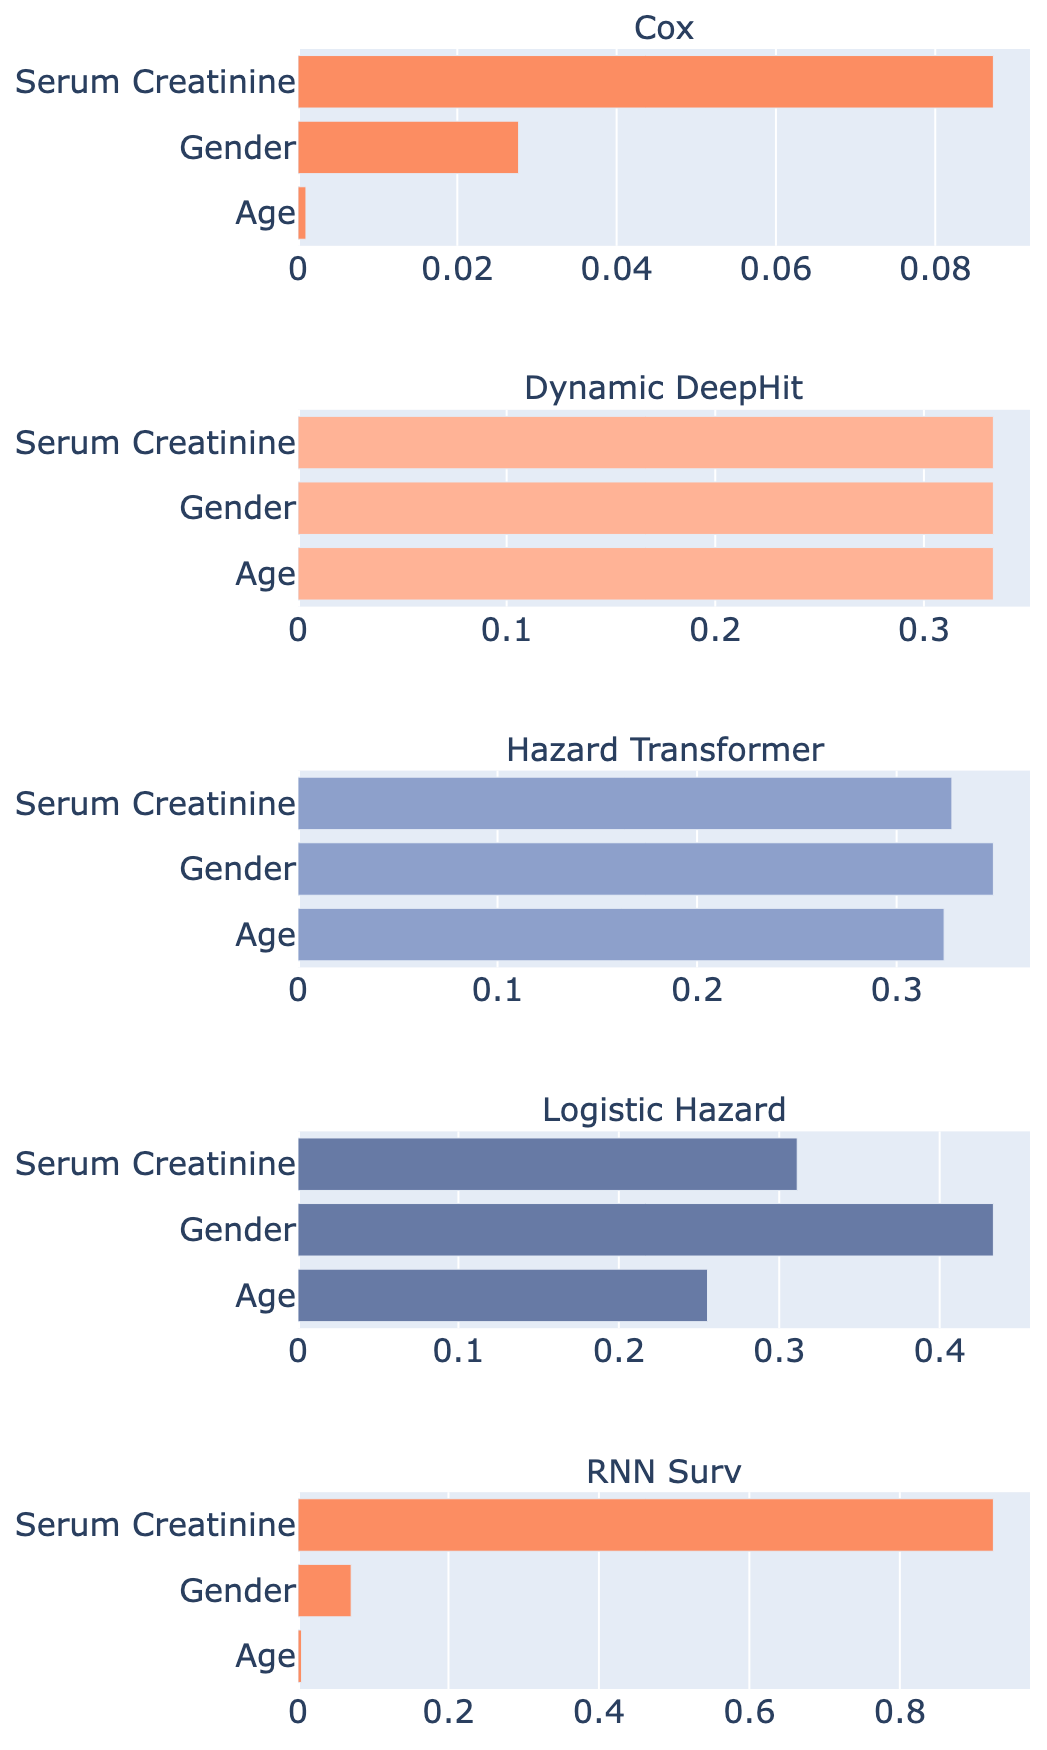
\includegraphics[width=0.5\textwidth]{figs/raw_feature_importance_individual.png}
    \caption{Feature Importance of the "Raw" Setting. We explore how directly inputting the individual components of the eGFR equation drives performance Here, we plot our Cox model's weight coefficients along with the gradient-based saliency maps \citep{simonyan2014deepinsideconvolutionalnetworks_cnn} across our neural baselines. We observe that serum creatinine is highly relevant across all models, but age and gender varies depending on the model.}
    \label{fig:Feature_Analysis_Raw}
    \vspace{-0.2cm}
\end{figure}

\begin{figure}[h!]
    \centering
    \vspace{-0.2cm}
    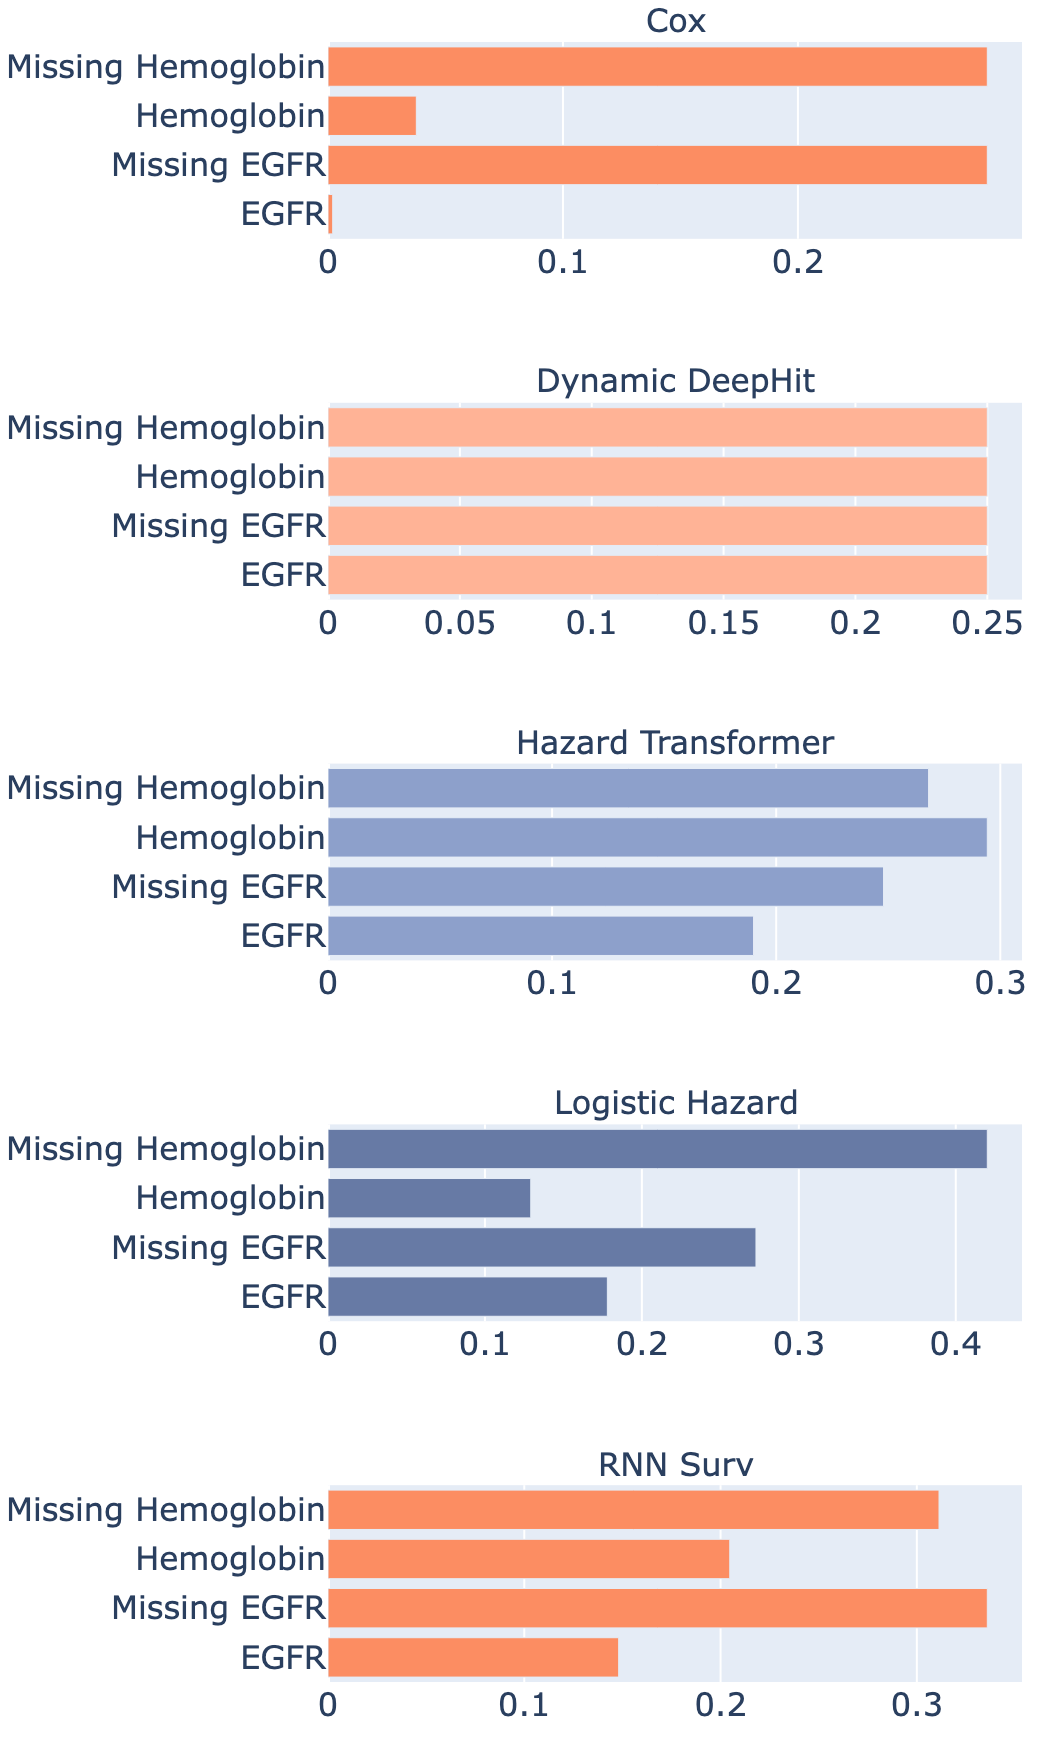
\includegraphics[width=0.5\textwidth]{figs/feature_importance_individual.png}
    \caption{Feature Importance Within The Heterogeneous Setting. We explore how (missing) features affect downstream performance by running a feature analysis. Here, we plot our Cox model's weight coefficients along with the gradient-based saliency maps \citep{simonyan2014deepinsideconvolutionalnetworks_cnn} with respect to each input feature across our neural baselines. We observe that missing features have a massive effect on model predictions.}
    \label{fig:Feature_Analysis_Hetero}
    \vspace{-0.2cm}
\end{figure}




% \subsection{Time Invariant Modeling}
% We first evaluated each model in a time-invariant setting, representing each patient by a single static snapshot. Overall discrimination was modest: no model achieved a C-index above 0.53 or an AUC above 0.54 (Table 2):contentReference[oaicite:1]{index=1}. DeepSurv achieved the highest C-index (0.526), whereas the Weibull model yielded the best AUC (0.537).

% \begin{table}[h]
%     \centering
%     \begin{tabular}{lcc}
%         \toprule
%         Model Name & C-Index & Brier score &AUC\\
%         \midrule
%         Cox & 0.503 & 0.504\\
%         DeepSurv & 0.526 & 0.46\\
%         GBSA & 0.497 & 0.505\\
%         SRF& 0.487&0.518\\
%         Weibull& 0.524&0.537\\
%     \end{tabular}
%     \caption{C-Index and AUC values for different models in time-invariant setting }
%     \label{tab:cindex_time_invariant}
% \end{table}
% \FloatBarrier

% \subsection{Time Variant Modeling}
% Incorporating longitudinal data markedly improved performance for certain models. Dynamic-DeepHit achieved exceptional discrimination (C-index = 0.733, AUC = 0.94), far surpassing both traditional Cox (C-index = 0.547, AUC = 0.542) and other deep methods (Table 3) :contentReference[oaicite:2]{index=2}. Time-variant Cox models showed slight gains over their time-invariant counterparts.

% \begin{table}[h]
%     \centering
%     \begin{tabular}{lcc}
%         \toprule
%         Model Name & C-Index & AUC\\
%         \midrule
%         Cox & 0.547 & 0.542\\
%         DynamicDeepHit & 0.733 & 0.94 \\
%         Hazard Transformer& 0.49& 0.504\\
%         RNNSurv& 0.67 & 0.681\\
%     \end{tabular}
%     \caption{C-Index and AUC values for different models}
%     \label{tab:cindex_time_variant}
% \end{table}
% \FloatBarrier

% \subsection{Heterogeneous}
% Dynamic-DeepHit remained the top performer (C-index = 0.69, AUC = 0.75), although with somewhat reduced accuracy compared to the fully observed setting (Table 4) :contentReference[oaicite:3]{index=3}. Traditional Cox models remained stable, whereas RNN-Surv show insignificant decrease in performance.

% \begin{table}[h]
%     \centering
%     \begin{tabular}{lcc}
%         \toprule
%         Model Name & C-Index & AUC\\
%         \midrule
%         Cox & 0.548 & 0.545\\  
%         RNNSurv & 0.656 & 0.668\\ 
%         DynamicDeepHit & 0.69 & 0.75\\
%         Hazard Transformer& 0.5& 0.505\\
%         \bottomrule
%  % RNNSurv& 0.344&0.668\\
%     \end{tabular}
%     \caption{C-Index and AUC values for different models}
%     \label{tab:cindex_heterogeneous}
% \end{table}
% \FloatBarrier

% \subsection{EGFR components}
% Finally, we replaced the composite eGFR feature with its constituent variables (age, sex, and serum creatinine) to evaluate whether the model could recover the same prognostic signal. Dynamic-DeepHit continued to lead (C-index = 0.69, AUC = 0.85), although RNNSurv performs slightly better (C-index = 0.693, AUC = 0.708).

% \begin{table}[h]
%     \centering
%     \begin{tabular}{lcc}
%         \toprule
%         Model Name & C-Index & AUC\\
%         \midrule
%         Cox & 0.381 & 0.358\\  
%         RNNSurv & 0.693 & 0.708\\ 
%         DynamicDeepHit & 0.69 & 0.85 \\
%         Hazard Transformer& 0.5& 0.5\\
%         \bottomrule
%  % RNNSurv& 0.307&0.708\\
%     \end{tabular}
%     \caption{C-Index and AUC values for different models}
%     \label{tab:cindex}
% \end{table}
% \FloatBarrier

% \begin{table}[htbp]
% \centering
% \begin{tabular}{lll}
%  & \multicolumn{2}{c}{\textbf{CKD stage 3-5 (n=10179)}}\\
% \hline
% \textbf{Characteristics} & \textbf{Non-ESRD (n=2,790)}& \textbf{ESRD (n=7,389)}\\
% \hline
% \multicolumn{3}{l}{\textbf{Demographics}} \\
% Age, years & 74.8 $\pm$ 12.5& 71.8 $\pm$ 13.7\\
% Gender & M: 1555, F: 1235& M: 4247, F: 3142\\
% \hline
% \multicolumn{3}{l}{\textbf{Hospitalization}} \\
% Number of admission & 47,441 & 6,773\\
% \hline
% \multicolumn{3}{l}{\textbf{Clinical Characteristics}} \\
% Hypertension, n (\%) & 1418 (50.8)& 4317 (58.4)\\
% Diabetes Mellitus, n (\%) & 565 (20.3)& 2288 (31.0)\\
% \hline
% \multicolumn{3}{l}{\textbf{Laboratory Parameters}} \\
% Serum Creatinine, mg/dL & 2.1 $\pm$ 2.0& 2.3 $\pm$ 1.7\\
% eGFR, mL/min/1.73m² & 46.4 $\pm$ 24.4& 41.0 $\pm$ 23.4\\
% Proteinuria, g/24h & 0.8 [2.3]& 0.5 [4.3]\\
% \hline
% \multicolumn{3}{l}{\textbf{Medication Use}} \\
% ACE Inhibitors or ARBs, n (\%) & 954 (34.2)& 3221 (43.6)\\
% \hline
% \multicolumn{3}{l}{\small *Proteinuria values presented as median [IQR]} \\
% \end{tabular}
% \caption{Baseline Characteristics of CKD Stage 3-5 Patients by ESRD Status. This analysis focuses exclusively on patients with chronic kidney disease stages 3-5 (n=10,179), stratified by whether they developed end-stage renal disease (ESRD) during follow-up. Continuous variables are presented as mean ± standard deviation, except for proteinuria which is presented as median with interquartile range due to its skewed distribution. We investigate a wide variety of useful features defined by \citep{zhong2017perspective_CKD_biomarkers} and more recently \citep{dana2024integratedmachinelearningsurvival_feature_analysis}. We investigate these features across time. We also investigate features that may not necessarily be omnipresent across all time points.}
% \label{tab:baseline_characteristics}
% \end{table}